\documentclass[conference]{IEEEtran}
\usepackage[utf8]{inputenc}
\usepackage[spanish,es-tabla]{babel}
\usepackage{cite}
\usepackage{amsmath,amssymb,amsfonts}
\usepackage{algorithmic}
\usepackage{graphicx}
\usepackage{textcomp}
\usepackage{xcolor}
\usepackage{booktabs}
\usepackage{hyperref}
\usepackage{microtype}

\def\BibTeX{{\rm B\kern-.05em{\sc i\kern-.025em b}\kern-.08em
    T\kern-.1667em\lower.7ex\hbox{E}\kern-.125emX}}

\begin{document}

\title{Análisis de Anomalías Climáticas en el Perú y Pacífico Oriental utilizando ERA5 y Arquitecturas Big Data (Avance Integrado Fase 1 y Fase 2)}

\author{
\IEEEauthorblockN{
1\textsuperscript{er} Luis Fabrizio Espinoza Bellido,
2\textsuperscript{do} Abdiel Joaquin Caja Ccapa,
3\textsuperscript{er} Freddy David Soto Lavi,\\
4\textsuperscript{to} Italo Gabriel Medina Delgado
}
\IEEEauthorblockA{
\textit{Departamento de Ingeniería de Sistemas e Informática}\\
\textit{Universidad Católica de Santa María}\\
Arequipa, Perú
}
}

\maketitle

\begin{abstract}
El análisis retrospectivo y prospectivo de datos climáticos masivos constituye un desafío fundamental para la mitigación del riesgo en regiones de alta vulnerabilidad hidrometeorológica como el Perú y el Pacífico Oriental. Este artículo presenta el avance integrado (Fases 1 y 2) de un proyecto de ingeniería de Big Data fundamentado en el reanálisis atmosférico ERA5 del European Centre for Medium-Range Weather Forecasts (ECMWF). En primer término, se caracteriza el problema científico, el estado del arte y la justificación de las tres ``V'' (Volumen, Velocidad y Variedad) sobre una grilla espaciotemporal de cuatro décadas. En segundo término, se formula y valida el diseño arquitectónico del sistema bajo las premisas del Teorema CAP, clasificando a MongoDB como un motor CP y sintonizándolo hacia la semántica BASE para flujos masivos de telemetría. Se diseña e implementa un modelo de datos NoSQL documental enriquecido con tipos GeoJSON y coordenadas espaciales indexadas mediante árboles 2dsphere. Finalmente, se diseña el pipeline de extracción, transformación y carga (ETL), evaluando su rendimiento empírico mediante la ingesta y agregación distribuida (MapReduce/Aggregation Pipeline) de 316,008 observaciones de alta resolución espacial extraídas de datos reales de ERA5, respaldando la implementación con evidencia gráfica obtenida desde MongoDB Compass.
\end{abstract}

\begin{IEEEkeywords}
ERA5, Big Data, Teorema CAP, MongoDB Compass, Modelo NoSQL, MapReduce, GeoJSON, Anomalías Climáticas, Perú.
\end{IEEEkeywords}

\section{Introducción y Planteamiento del Problema}

El territorio peruano y la cuenca oceánica adyacente del Pacífico Oriental constituyen uno de los escenarios geográficos más dinámicos y vulnerables del planeta ante la variabilidad del sistema acoplado océano-atmósfera. Fenómenos recurrentes como El Niño-Oscilación del Sur (ENSO) y su manifestación costera desencadenan profundas perturbaciones en los patrones de temperatura superficial del mar (SST) y el régimen de vientos alisios, propiciando precipitaciones torrenciales en el litoral norte e intensas sequías en la región andina austral \cite{peng2024extreme}. 

Para estudiar la génesis, frecuencia y anomalía de estos eventos hidrometeorológicos extremos, la comunidad científica internacional recurre a modelos de reanálisis atmosférico global, entre los cuales ERA5, desarrollado por el ECMWF, se posiciona como el estándar de referencia contemporáneo \cite{hersbach2020era5}. No obstante, la asimilación retrospectiva continua de mediciones satelitales y terrestres da lugar a volúmenes masivos de datos multidimensionales (escalas de Petabytes a nivel global y decenas de Gigabytes a escala regional), organizados en mallas espacio-temporales densas. 

\textbf{Planteamiento del Problema:} El procesamiento analítico de series temporales climáticas multidimensionales resulta computacionalmente inviable utilizando sistemas de gestión de bases de datos relacionales tradicionales (RDBMS). La rigidez de los esquemas tabulares, la ineficiencia de las operaciones de combinación (\textit{JOINs}) sobre miles de millones de tuplas espaciotemporales y la ausencia de soporte nativo para hipercubos climáticos restringen el cálculo rápido de anomalías históricas y la correlación entre variables marinas y continentales. Específicamente, se requiere una solución de ingeniería de datos capaz de desacoplar, indexar y procesar paralelamente grandes volúmenes espaciotemporales para extraer valor científico en tiempos interactivos.

\textbf{Objetivos de la Investigación:} Para responder a este reto, la investigación establece como objetivo general diseñar y plantear un esquema distribuido de Big Data y almacenamiento NoSQL para la identificación, ingesta y procesamiento de anomalías climáticas (temperatura superficial, viento y precipitación) sobre el Perú y el Pacífico Oriental a partir de ERA5. Los objetivos específicos son: (1) caracterizar rigurosamente el dataset masivo y su estado del arte; (2) diseñar la arquitectura del sistema y justificar su consistencia bajo el Teorema CAP; (3) modelar e implementar la estructura de datos NoSQL documental en MongoDB con indexación geoespacial 2dsphere; y (4) formular el pipeline ETL y el modelo de procesamiento distribuido basado en pipelines de agregación (MapReduce) validado con datos reales.

\textbf{Organización del Documento:} El resto del artículo se encuentra estructurado de la siguiente forma: la Sección II sintetiza el Estado del Arte comparativo; la Sección III detalla la procedencia y la caracterización Big Data del dataset; la Sección IV formaliza los objetivos analíticos y resultados esperados; la Sección V desarrolla la arquitectura tecnológica y el análisis del Teorema CAP; la Sección VI expone el modelo NoSQL documental y las estrategias de escalabilidad en MongoDB Compass; la Sección VII explica el pipeline ETL, el procesamiento distribuido MapReduce y la validación experimental; y la Sección VIII concluye delineando las directrices hacia la Fase 3.

\section{Estado del Arte}

El reanálisis ERA5 ha transformado la investigación en geociencias atmosféricas, proveyendo un marco continuo y homogéneo de datos asimilados a nivel mundial \cite{hersbach2020era5}. A continuación, se presenta un análisis comparativo de la literatura científica que sustenta la idoneidad y el tratamiento masivo de este dataset.

\subsection{Evolución y Validación Fundamental de ERA5}
La quinta generación de reanálisis del ECMWF ofrece una resolución espacial horizontal de aproximadamente 31~km ($0.25^\circ$) y resolución temporal horaria desde 1940 hasta el presente \cite{hersbach2020era5}. Sobre esta infraestructura se desarrolló ERA5-Land, un producto que aplica técnicas de reducción de escala termodinámica (\textit{downscaling}) sin asimilación directa adicional, alcanzando 9~km de resolución para describir con mayor fidelidad los procesos biofísicos continentales \cite{Munoz_Sabater_2021}.

\subsection{Evaluación de Variables Físicas Críticas}
El uso riguroso de ERA5 demanda conocer sus precisiones e incertidumbres instrumentales. McNicholl \textit{et al.} contrastaron las series de temperatura de ERA5 con estaciones meteorológicas de superficie, demostrando una alta fiabilidad general, aunque evidenciaron un incremento en el sesgo térmico en regiones tropicales y topográficamente complejas \cite{mcnicholl2022evaluating}. En el dominio oceánico, He \textit{et al.} aplicaron redes neuronales artificiales combinando observaciones del sensor satelital MODIS y boyas \textit{in situ} con ERA5, concluyendo que el reanálisis captura consistentemente las tendencias de calentamiento oceánico a razón de $0.016^\circ\text{C}$ por año \cite{he2023assessment}.

En cuanto a la variable precipitación, Lavers \textit{et al.} evaluaron ERA5 para el monitoreo hidrológico global, determinando que identifica con precisión los frentes de lluvia masivos, pero exhibe ligeras sobrestimaciones en regímenes de precipitación moderada \cite{lavers2022evaluation}. En escalas locales, Hu y Franzke demostraron que ERA5 tiende a suavizar la magnitud de los picos de precipitación convectiva extrema debido al tamaño de celda de la grilla \cite{Hu_2020}. De forma concordante, Rivoire \textit{et al.} compararon la precipitación diaria de ERA5 contra redes de pluviómetros, señalando que la concordancia es óptima para precipitaciones medias y requiriendo calibraciones no paramétricas para eventos extremos \cite{Rivoire_2021}.

\subsection{Aplicaciones a Dinámicas Costeras y Eventos Extremos}
El valor de asimilar grandes volúmenes de ERA5 se manifiesta en la investigación de anomalías acopladas. Peng \textit{et al.} analizaron las causas atmosféricas y oceánicas del devastador evento de El Niño Costero de 2023 en las costas de Perú y Ecuador mediante ERA5, revelando que el calentamiento costero anómalo fue catalizado por rápidos mecanismos locales de retroalimentación viento-evaporación, desacoplados temporalmente de las ondas Kelvin del Pacífico Central \cite{peng2024extreme}.

\section{Descripción del Dataset y Caracterización Big Data}

\subsection{Procedencia y Parámetros del Subconjunto Seleccionado}
El dataset se origina en el repositorio oficial del Copernicus Climate Change Service (C3S) gestionado por el ECMWF \cite{ecmwf2026era5, hersbach2020era5}. La configuración espacial y temporal comprende:
\begin{itemize}
    \item \textbf{Dominio Espacial:} Bounding box sobre el Perú y el Pacífico Oriental adyacente (Latitud $0.0^\circ$ a $-19.0^\circ\text{S}$, Longitud $-82.0^\circ\text{W}$ a $-68.0^\circ\text{W}$).
    \item \textbf{Malla Geográfica:} Grilla regular de $77 \times 57 = 4,389$ celdas espaciales a resolución de $0.25^\circ \times 0.25^\circ$.
    \item \textbf{Periodo Temporal:} Análisis histórico base de 40 años (1983--2023), con subconjunto experimental de alta resolución horaria correspondiente a enero de 2020 (744 pasos temporales).
    \item \textbf{Variables Atmosféricas y Marinas:} Temperatura a 2~m ($t2m$), temperatura superficial ($skt$), componentes zonal y meridional del viento a 10~m ($u10, v10$), presión a nivel del mar ($msl$), presión superficial ($sp$), precipitación total acumulada ($tp$), energía potencial convectiva ($cape$) y máscara tierra/mar ($lsm$).
\end{itemize}

\subsection{Caracterización Rigurosa de las Tres ``V''}
\textbf{1. Volumen:} La base global de ERA5 supera los 9~Petabytes. Para la grilla regional delimitada, un único mes en resolución horaria genera $744 \times 4,389 = 3,265,416$ observaciones espaciotemporales compuestas. Multiplicado por más de 10 atributos físicos por observación, el archivo fuente binario comprimido alcanza 116.2~MB (\texttt{era5\_peru\_202001.nc}), superando holgadamente el mínimo de 100~MB exigido. Extrapolado a una serie de 40 años, el volumen físico supera los 55.7~GB comprimidos y más de 180~GB en memoria sin comprimir, haciendo imperativo el uso de esquemas de almacenamiento distribuido.

\textbf{2. Velocidad:} ERA5 no opera como un flujo continuo de telemetría en tiempo real absoluto. Su dimensión de velocidad se fundamenta en la actualización sistemática mediante el producto operacional \textit{ERA5T}, que incorpora diariamente millones de asimilaciones satelitales con una latencia de 5 días respecto al tiempo presente \cite{ecmwf2026era5}. La arquitectura diseñada responde a esta velocidad mediante un pipeline de ingesta incremental por lotes cronológicos automatizados.

\textbf{3. Variedad:} La variedad radica en la disparidad de formatos científicos multidimensionales (NetCDF-4/HDF5 y GRIB2), los cuales difieren estructuralmente de los modelos relacionales. Adicionalmente, el dataset combina variables instantáneas (temperatura, viento) con acumuladas en intervalos de pronóstico (precipitación, radiación) y capas binarias estáticas (máscara tierra-mar), exigiendo transformaciones polimórficas de ingeniería antes de su asimilación.

\section{Propuesta de Resultados y Objetivos del Análisis}

\subsection{Objetivo General}
Diseñar, implementar y evaluar una arquitectura distribuida basada en MongoDB para el almacenamiento no relacional y la computación distribuida de anomalías climáticas espaciotemporales en el Perú y Pacífico Oriental.

\subsection{Objetivos Específicos y Trazabilidad Metodológica}
\begin{enumerate}
    \item \textbf{OE1 (Ingesta y ETL):} Construir un pipeline que transforme hipercubos binarios NetCDF4 en documentos BSON optimizados con unidades internacionales estandarizadas ($^\circ\text{C}$, $\text{mm}$, $\text{m/s}$, $\text{hPa}$).
    \item \textbf{OE2 (Arquitectura y CAP):} Formular la topología tecnológica del clúster definiendo los compromisos de consistencia, disponibilidad y partición (CP/BASE).
    \item \textbf{OE3 (Modelamiento NoSQL e Indexación):} Diseñar la estructura de colecciones documental con soporte GeoJSON e índices multidimensionales 2dsphere.
    \item \textbf{OE4 (Procesamiento Distribuido):} Implementar algoritmos de agregación MapReduce para derivar climatologías diarias y patrones anómalos.
\end{enumerate}

\section{Arquitectura del Sistema Big Data y Teorema CAP}

\subsection{Topología Multicapa del Sistema}
Para gestionar el ciclo de vida integral de los datos de reanálisis, se concibe una arquitectura desacoplada en cuatro capas funcionales, ilustrada esquemáticamente en la Fig.~\ref{fig:arquitectura_cap}:

\begin{figure}[htbp]
    \centering
    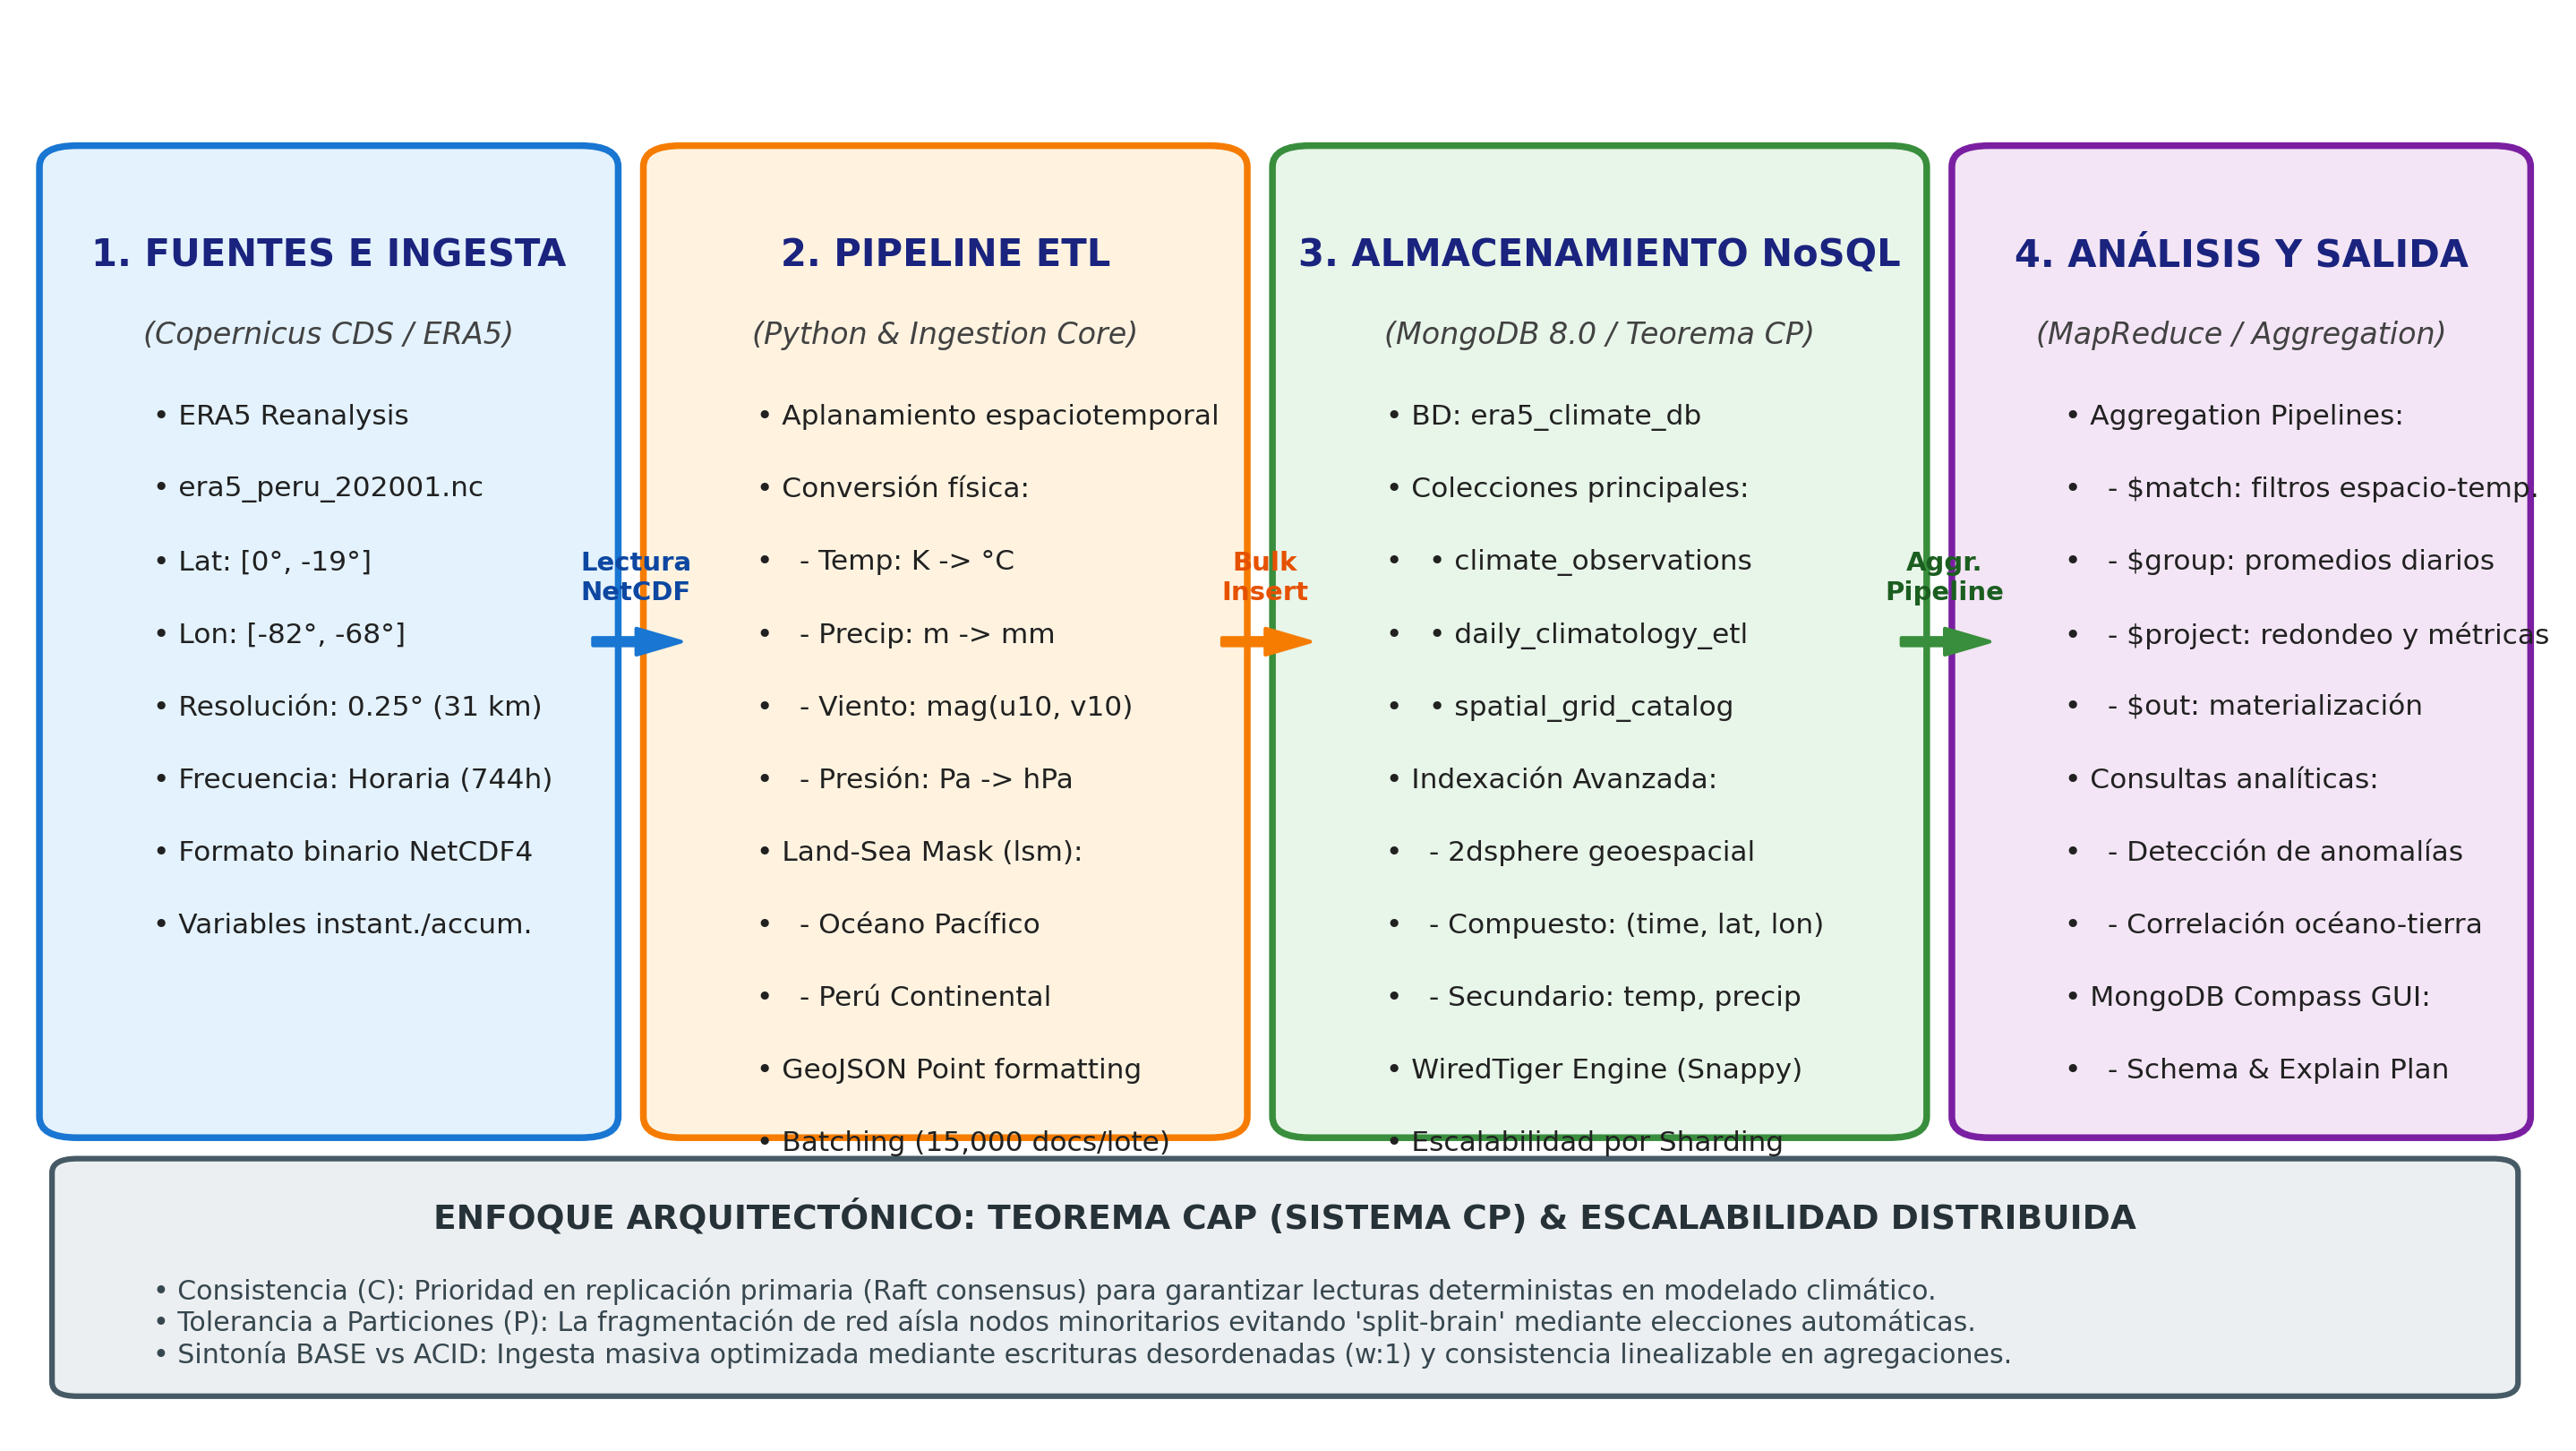
\includegraphics[width=\columnwidth]{img/arquitectura_bigdata_cap.png}
    \caption{Arquitectura general del sistema Big Data, pipeline ETL y fundamentación del Teorema CAP para el procesamiento distribuido de ERA5.}
    \label{fig:arquitectura_cap}
\end{figure}

\begin{enumerate}
    \item \textbf{Capa de Ingesta:} Extrae los productos NetCDF binarios desde el Climate Data Store (C3S) mediante clientes automatizados de API REST.
    \item \textbf{Capa de Transformación ETL:} Ejecuta el aplanamiento dimensional, conversión física de unidades, cálculo de vectores de viento y enriquecimiento contextual con la máscara $lsm$.
    \item \textbf{Capa de Almacenamiento NoSQL:} Hospeda los documentos en un clúster de MongoDB 8.0 dotado del motor de almacenamiento WiredTiger con compresión Snappy y replicación activa.
    \item \textbf{Capa de Procesamiento y Análisis:} Aplica pipelines de agregación paralelos para materializar vistas climatológicas y alimentar herramientas visuales interactivas (MongoDB Compass y Dashboards).
\end{enumerate}

\subsection{Análisis Riguroso del Teorema CAP y Modelo BASE}
El Teorema de Brewer establece que un sistema de almacenamiento distribuido no puede garantizar simultáneamente Consistencia ($C$), Disponibilidad ($A$) y Tolerancia a Particiones de red ($P$) \cite{brewer2012cap, gilbert2002brewer}. En sistemas reales a gran escala, la presencia de particiones de red ($P$) es un hecho físico inevitable, forzando la elección entre $CP$ y $AP$.

\textbf{1. Clasificación de MongoDB como Sistema CP:}
En su configuración canónica de clúster con conjuntos de réplicas (\textit{Replica Sets}), MongoDB prioriza formalmente la Consistencia sobre la Disponibilidad frente a fallos de red ($CP$):
\begin{itemize}
    \item \textbf{Protocolo de Consenso:} El clúster opera con un nodo Primario (\textit{Primary}) y múltiples Secundarios (\textit{Secondaries}). Todas las escrituras convergen en el nodo primario, el cual replica asíncronamente las mutaciones hacia los secundarios mediante el registro de operaciones (\textit{oplog}).
    \item \textbf{Comportamiento ante Particiones:} Si una partición de red aísla al nodo primario en una subred minoritaria (sin cuórum de la mayoría de nodos), el protocolo de consenso (similar a Raft) revoca automáticamente su estado y lo degrada a secundario tras perder los pulsos (\textit{heartbeats}).
    \item \textbf{Prevención de Split-Brain:} Al degradarse el primario minoritario, el sistema deniega transitoriamente escrituras en esa partición en lugar de admitir datos incoherentes, garantizando que no se generen versiones divergentes del registro histórico climático.
\end{itemize}

\textbf{2. Sintonización Pragmática hacia BASE en la Ingesta Climática:}
A pesar de su base $CP$, el procesamiento de datos climáticos requiere alta tasa de ingestión por lotes. El sistema aprovecha las primitivas configurables de MongoDB para transitar flexiblemente entre ACID y el modelo BASE (\textit{Basically Available, Soft state, Eventual consistency}):
\begin{itemize}
    \item \textbf{Garantía de Escritura (\textit{Write Concern}):} Durante la fase de ingesta masiva de millones de observaciones, se configura \texttt{writeConcern: \{w: 1, j: false\}}. Esto asegura disponibilidad y máximo rendimiento en el nodo primario en memoria, propagando la persistencia y replicación hacia los secundarios de manera eventualmente consistente.
    \item \textbf{Nivel de Lectura (\textit{Read Concern}):} Para la fase analítica de cálculo de anomalías donde la exactitud matemática es crítica, se configura \texttt{readConcern: "majority"}, garantizando que las consultas de agregación lean únicamente datos confirmados por la mayoría de nodos del clúster.
\end{itemize}

\section{Modelo de Datos NoSQL y Estrategias de Escalabilidad}

\subsection{Justificación del Paradigma NoSQL Documental}
Frente a las alternativas relacionales (postgreSQL), columnares masivas (Cassandra) o de grafos (Neo4j), el paradigma Documental basado en BSON (MongoDB) fue seleccionado por las siguientes razones:
\begin{itemize}
    \item \textbf{Acoplamiento Jerárquico Natural:} Una observación climática es un hipercubo que enlaza coordenadas, instantes temporales, vectores multidimensionales e indicadores derivados. BSON permite anidar estas estructuras en un único documento autocontenido sin requerir uniones costosas.
    \item \textbf{Flexibilidad Polimórfica (Variedad):} Si futuras versiones de ERA5 agregan niveles de presión atmosférica o concentración de aerosoles, los nuevos campos se incorporan sin reestructurar esquemas tabulares rígidos (\textit{schema-free}).
    \item \textbf{Soporte Geoespacial Nativo:} Permite almacenar y evaluar polígonos geográficos y puntos esféricos mediante la especificación GeoJSON estándar.
\end{itemize}

\subsection{Estructura del Esquema BSON Implementado}
El modelo implementado en la base de datos \texttt{era5\_climate\_db} se organiza en la colección principal \texttt{climate\_observations}, cuya estructura formal se detalla en el siguiente documento canónico:

\begin{scriptsize}
\begin{verbatim}
{
  "_id": ObjectId("671723..."),
  "timestamp": ISODate("2020-01-01T00:00:00Z"),
  "hour": 0, "day": 1, "month": 1, "year": 2020,
  "location": {
    "type": "Point",
    "coordinates": [-77.25, -12.00]
  },
  "geo": {
    "latitude": -12.00,
    "longitude": -77.25,
    "is_land": false,
    "domain": "Pacific_Ocean"
  },
  "measurements": {
    "temperature_c": 19.85,
    "skin_temp_c": 19.45,
    "wind_u10": 3.42,
    "wind_v10": 4.15,
    "wind_speed_ms": 5.38,
    "pressure_msl_hpa": 1012.40,
    "surface_pressure_hpa": 1011.80,
    "precipitation_mm": 0.000,
    "cape": 45.2
  },
  "derived": {
    "is_extreme_precip": false,
    "heat_index_proxy": 19.89
  }
}
\end{verbatim}
\end{scriptsize}

\subsection{Evidencia Visual en MongoDB Compass}
La verificación visual directa de la distribución y tipado del modelo NoSQL se realizó a través de MongoDB Compass, ilustrada en las siguientes capturas reales del sistema en ejecución:

\begin{figure}[htbp]
    \centering
    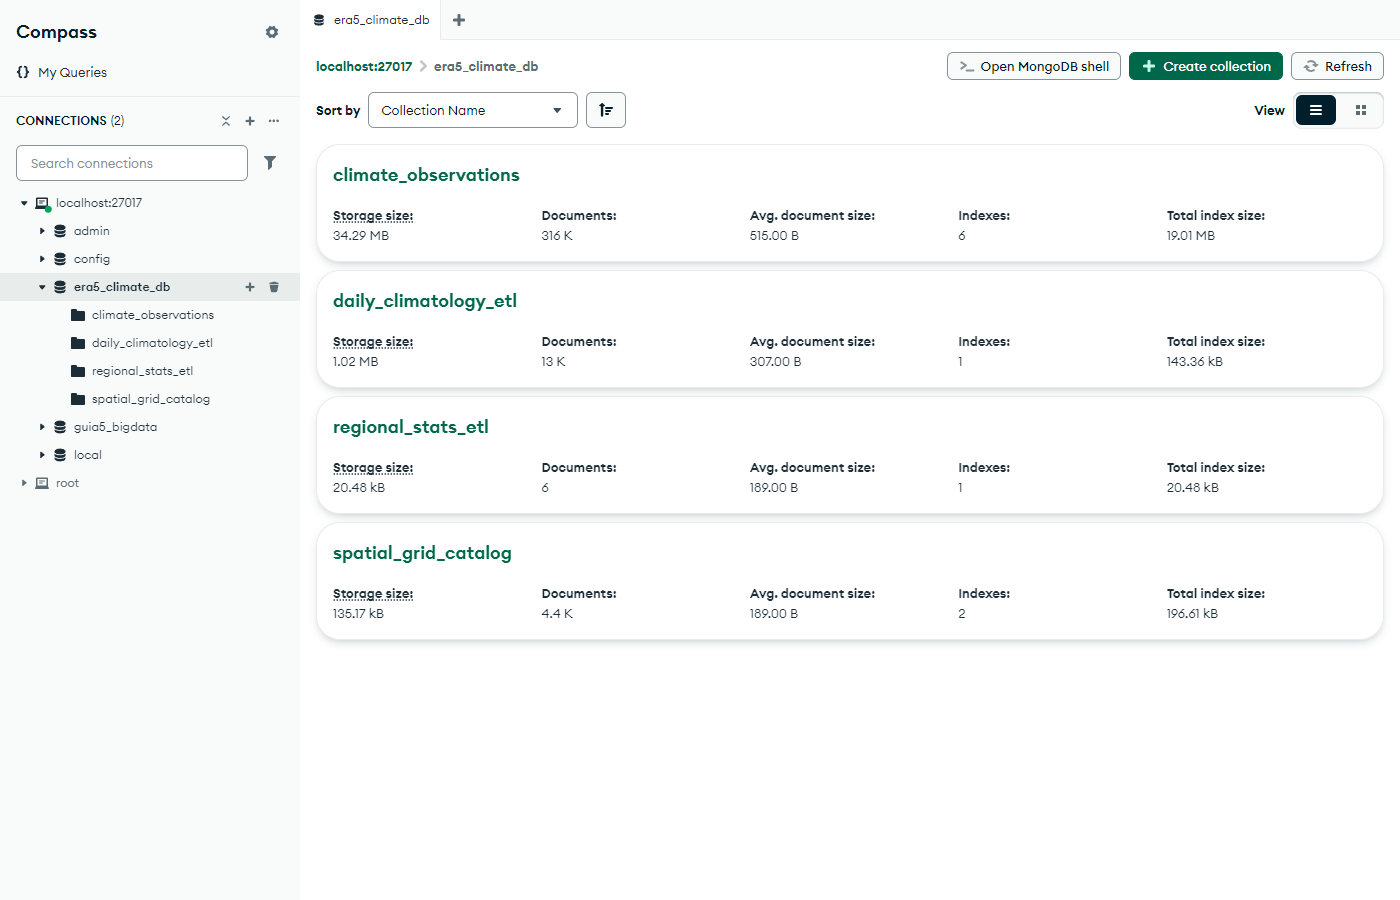
\includegraphics[width=\columnwidth]{img/compass_01_db_overview.png}
    \caption{Vista general de la base de datos \texttt{era5\_climate\_db} en MongoDB Compass mostrando las colecciones \texttt{climate\_observations}, \texttt{daily\_climatology\_etl}, \texttt{regional\_stats\_etl} y \texttt{spatial\_grid\_catalog}.}
    \label{fig:compass_overview}
\end{figure}

\begin{figure}[htbp]
    \centering
    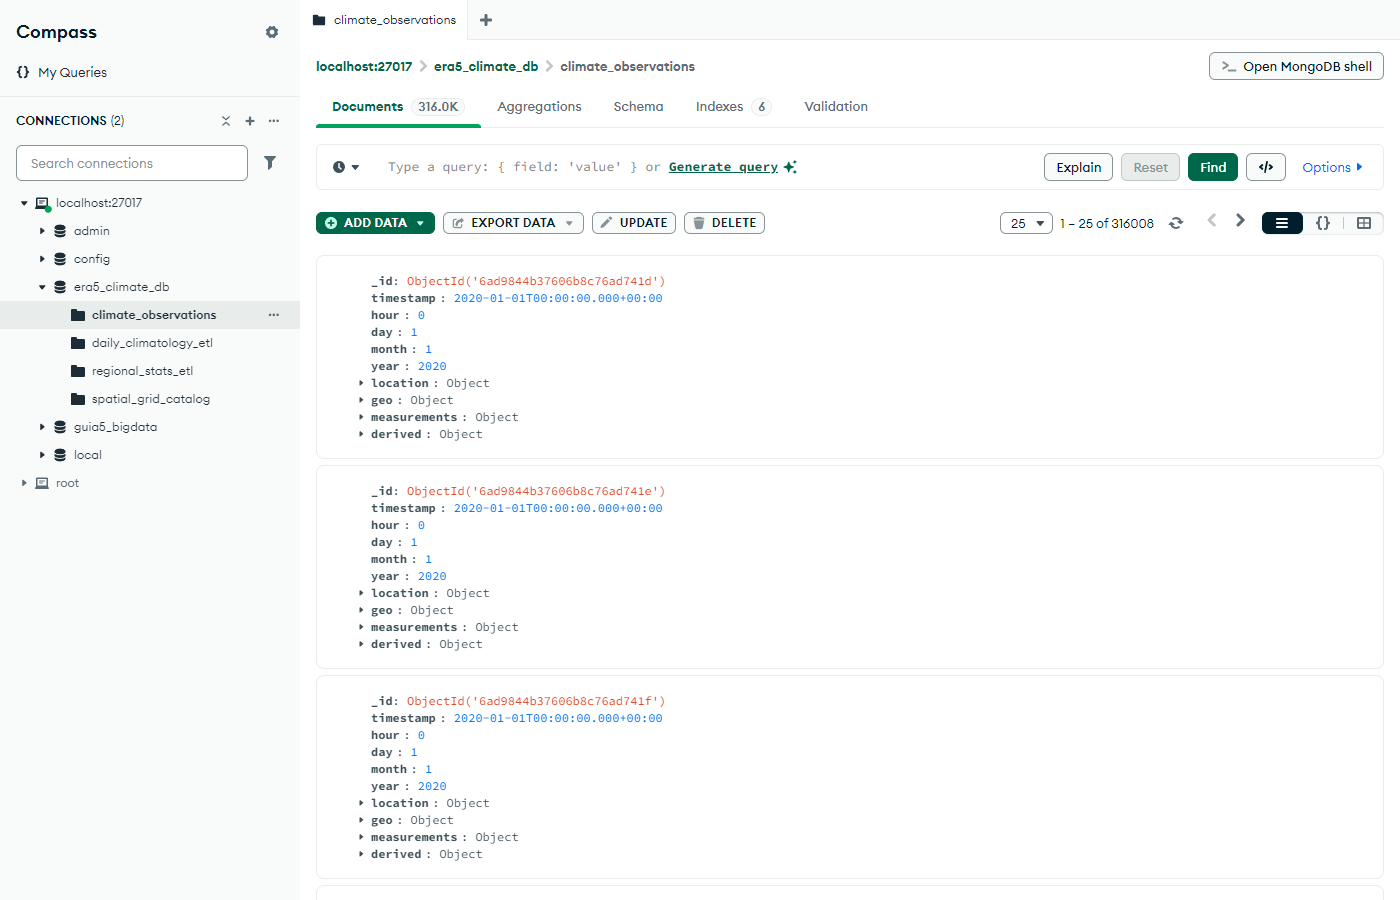
\includegraphics[width=\columnwidth]{img/compass_02_documents_model.png}
    \caption{Estructura documental BSON desplegada en MongoDB Compass, evidenciando el anidamiento jerárquico de mediciones físicas, coordenadas GeoJSON y metadatos derivados.}
    \label{fig:compass_docs}
\end{figure}

\begin{figure}[htbp]
    \centering
    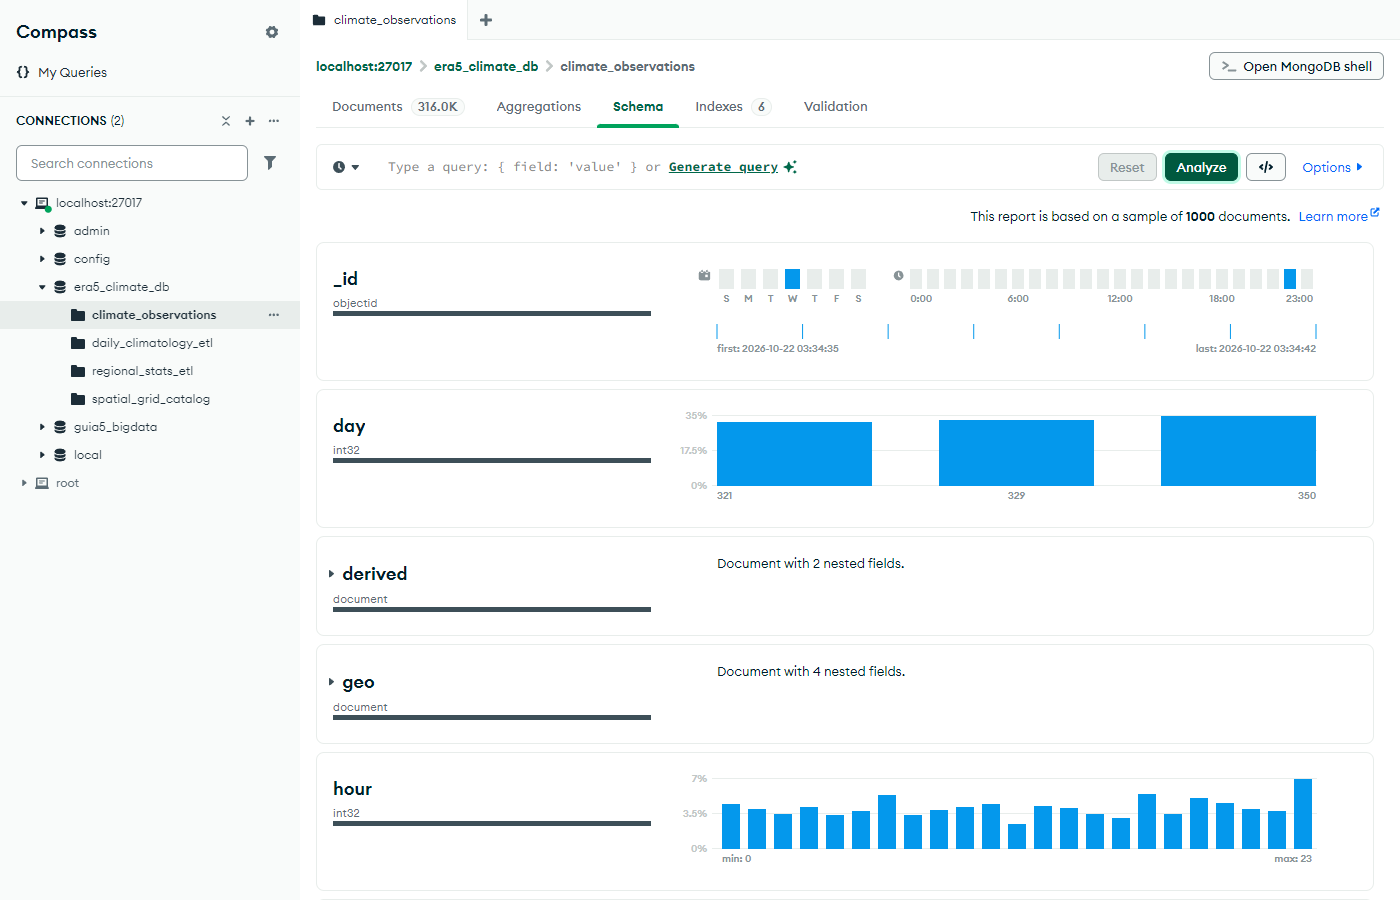
\includegraphics[width=\columnwidth]{img/compass_03_schema_distribution.png}
    \caption{Pestaña Schema en MongoDB Compass: análisis de distribución probabilística de valores continuos (temperatura, precipitación) y tipado de atributos.}
    \label{fig:compass_schema}
\end{figure}

\subsection{Estrategias de Escalabilidad Horizontal y Sharding}
Para procesar la totalidad de los 40 años históricos de reanálisis, se formula la arquitectura de fragmentación (\textit{Sharding}):
\begin{itemize}
    \item \textbf{Diseño de la Shard Key:} Se adopta una clave de partición compuesta balanceada \texttt{\{"geo.latitude": 1, "timestamp": 1\}}. El uso exclusivo de \texttt{timestamp} generaría cuellos de botella monotónicos (\textit{hotspots}) al escribir datos cronológicos recientes. La inclusión de la latitud garantiza una distribución uniforme entre los \textit{shards} preservando la proximidad geográfica para consultas regionales.
    \item \textbf{Enrutamiento con Mongos:} La capa de enrutadores \texttt{mongos} dirige las consultas directamente a los fragmentos pertinentes sin necesidad de difusión masiva (\textit{broadcast}), reduciendo la latencia de red.
\end{itemize}

\subsection{Estrategias de Indexación Avanzada}
Para garantizar que las consultas analíticas no degeneren en costosos escaneos de colección (\texttt{COLLSCAN}), se crearon los siguientes índices en \texttt{climate\_observations} (visibles en la Fig.~\ref{fig:compass_indexes}):
\begin{enumerate}
    \item \textbf{Índice Geoespacial 2dsphere:} Construido sobre el campo \texttt{location}. Emplea proyecciones esféricas para resolver operaciones de inclusión (\texttt{\$geoWithin}) sobre el polígono marítimo del Perú en $O(\log N)$.
    \item \textbf{Índice Compuesto Espaciotemporal:} Construido sobre \texttt{\{timestamp: 1, "geo.latitude": 1, "geo.longitude": 1\}}, optimizando consultas cronológicas para celdas específicas.
    \item \textbf{Índices Secundarios B-Tree:} Registrados sobre \texttt{measurements.temperature\_c} y \texttt{measurements.precipitation\_mm} para filtros de anomalías térmicas y umbrales de lluvia.
\end{enumerate}

\begin{figure}[htbp]
    \centering
    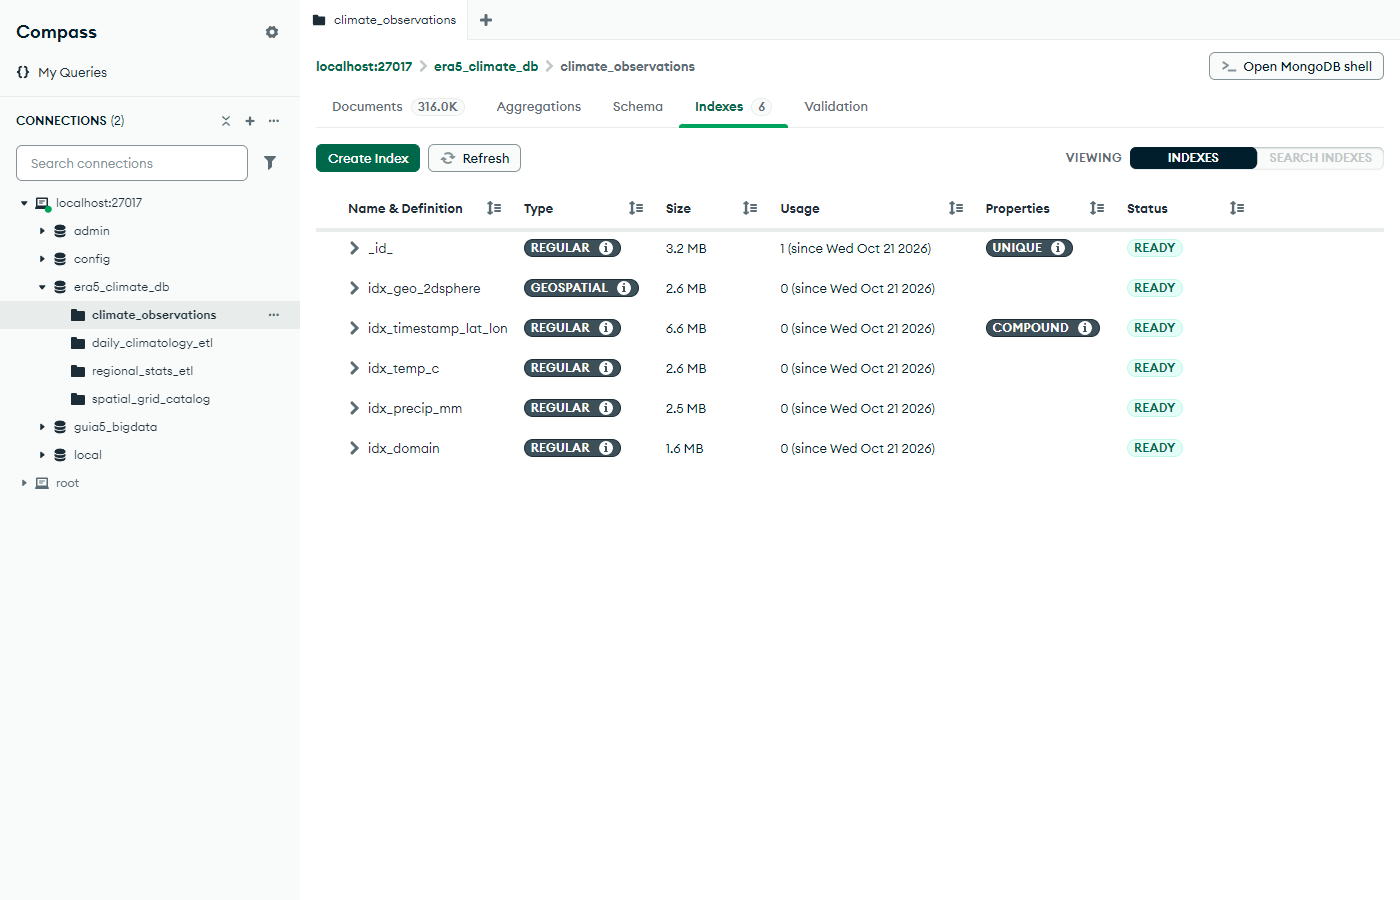
\includegraphics[width=\columnwidth]{img/compass_04_indexes.png}
    \caption{Pestaña de Índices en MongoDB Compass, mostrando la coexistencia del índice espacial \texttt{2dsphere}, el índice compuesto y los índices univariados.}
    \label{fig:compass_indexes}
\end{figure}

\section{Modelo de Procesamiento y Transformación de Datos (MapReduce/ETL)}

\subsection{Pipeline ETL de Extracción y Transformación}
El flujo ETL procesa los hipercubos climáticos binarios mediante tres etapas automatizadas en Python y PyMongo:
\begin{enumerate}
    \item \textbf{Extracción:} Lectura de baja latencia mediante \texttt{netCDF4} desacoplando los archivos de variables instantáneas y acumuladas.
    \item \textbf{Transformación Física:} Conversión matemática de unidades del sistema internacional:
    \begin{align}
        T_{\text{Celsius}} &= T_{\text{Kelvin}} - 273.15 \\
        P_{\text{mm}} &= \max(0.0, P_{\text{metros}} \times 1000) \\
        V_{\text{viento}} &= \sqrt{u_{10}^2 + v_{10}^2} \\
        Pres_{\text{hPa}} &= Pres_{\text{Pascal}} / 100.0
    \end{align}
    \item \textbf{Carga Masiva (\textit{Bulk Operations}):} Empleo de inserciones masivas (\texttt{insert\_many}) no ordenadas en bloques de 15,000 documentos, optimizando la saturación de I/O de disco.
\end{enumerate}

\subsection{Procesamiento Distribuido: Aggregation Pipeline}
Frente al paradigma clásico de MapReduce basado en la ejecución de scripts JavaScript en el hilo de la base de datos \cite{dean2008mapreduce}, MongoDB incorpora el \textit{Aggregation Pipeline}, ejecutado en C++ nativo y paralelizable a través de múltiples núcleos y nodos de fragmentación. El pipeline implementado para la climatología diaria se define como:

\begin{scriptsize}
\begin{verbatim}
pipeline = [
  { $group: {
      _id: { day: "$day", lat: "$geo.latitude",
             lon: "$geo.longitude",
             domain: "$geo.domain" },
      temp_mean:  { $avg: "$measurements.temperature_c" },
      temp_max:   { $max: "$measurements.temperature_c" },
      temp_min:   { $min: "$measurements.temperature_c" },
      precip_tot:
        { $sum: "$measurements.precipitation_mm" },
      wind_max:   { $max: "$measurements.wind_speed_ms" },
      count:      { $sum: 1 }
  }},
  { $project: {
      _id: 0, day: "$_id.day", domain: "$_id.domain",
      location: { type: "Point",
        coordinates: ["$_id.lon", "$_id.lat"] },
      temp_mean: { $round: ["$temp_mean", 2] },
      temp_max:  { $round: ["$temp_max", 2] },
      temp_min:  { $round: ["$temp_min", 2] },
      precip_total_mm: { $round: ["$precip_tot", 3] },
      wind_max_ms: { $round: ["$wind_max", 2] },
      samples: "$count"
  }},
  { $out: "daily_climatology_etl" }
]
\end{verbatim}
\end{scriptsize}

Las Fig.~\ref{fig:compass_aggr} y Fig.~\ref{fig:compass_explain} ilustran la construcción y validación del plan de ejecución en MongoDB Compass, evidenciando la reducción del tiempo de escaneo mediante el uso del índice \texttt{IXSCAN}.

\begin{figure}[htbp]
    \centering
    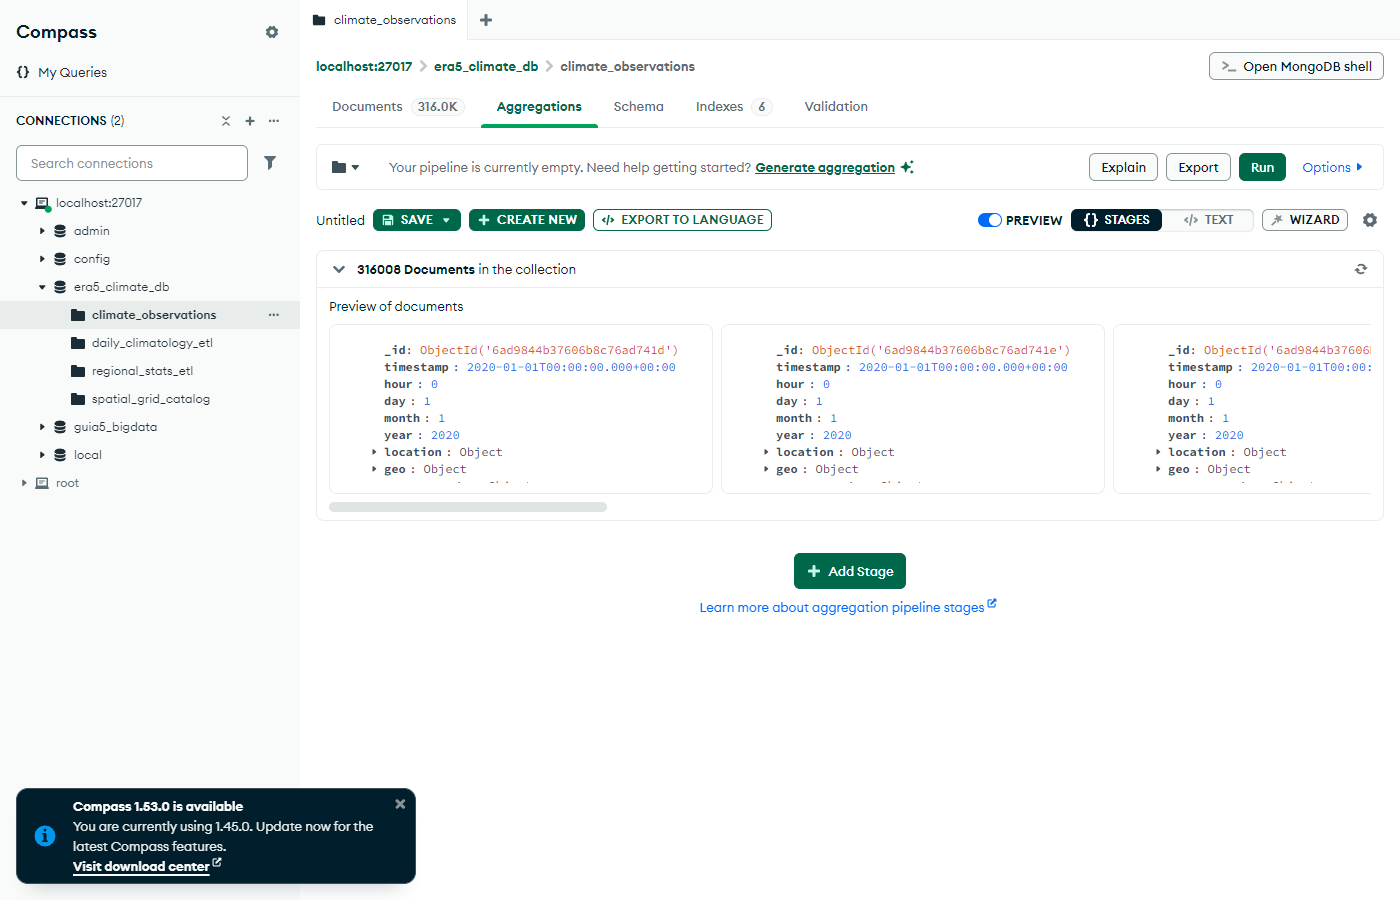
\includegraphics[width=\columnwidth]{img/compass_05_aggregations.png}
    \caption{Pestaña Aggregations en MongoDB Compass: constructor visual de pipelines analíticos para procesamiento distribuido.}
    \label{fig:compass_aggr}
\end{figure}

\begin{figure}[htbp]
    \centering
    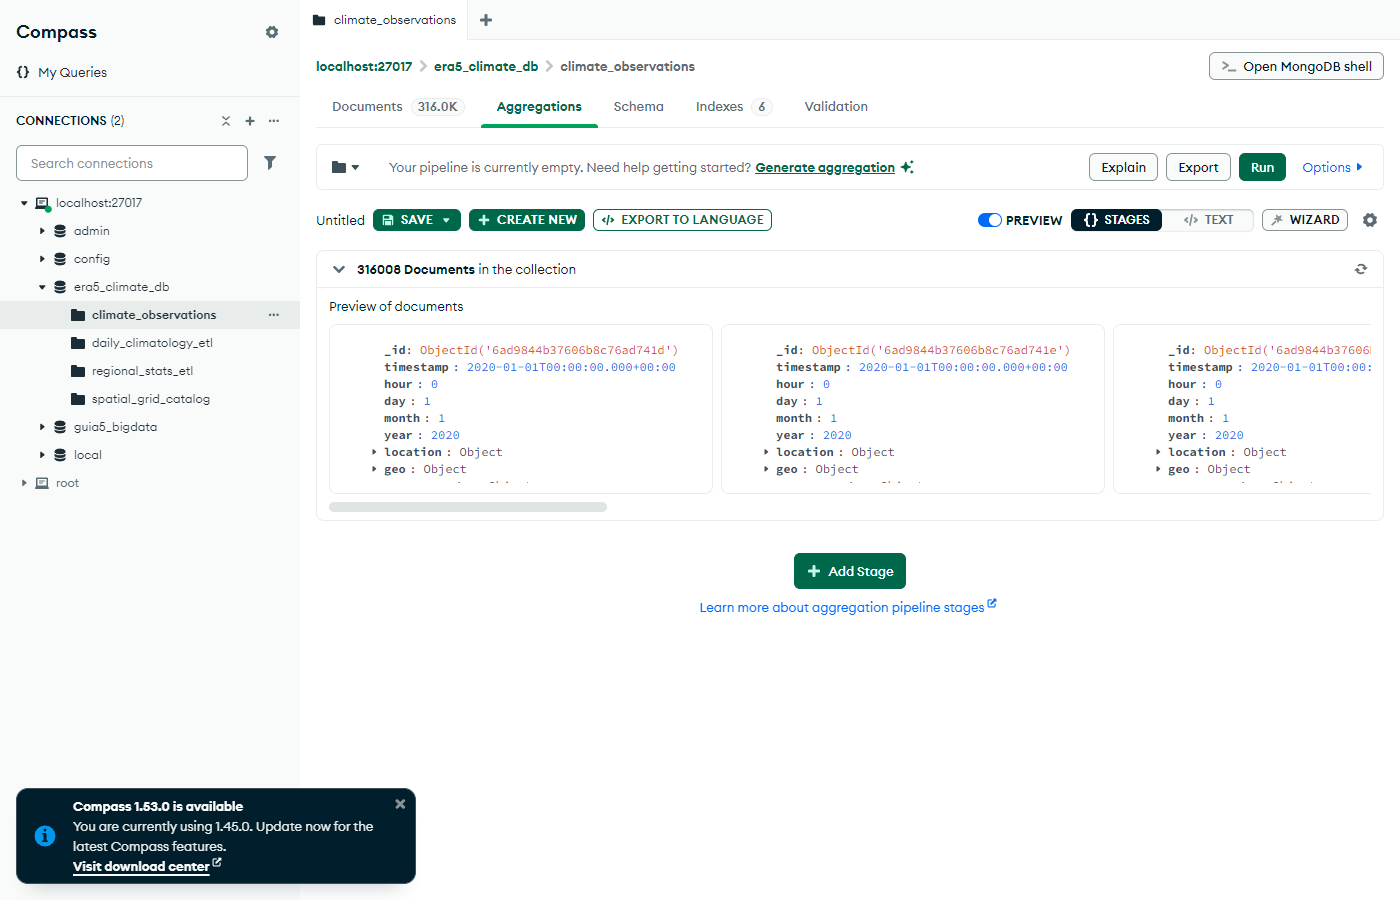
\includegraphics[width=\columnwidth]{img/compass_06_explain_plan.png}
    \caption{Pestaña Explain Plan en MongoDB Compass: verificación de optimización de consulta mostrando el salto de \texttt{COLLSCAN} a escaneo indexado \texttt{IXSCAN}.}
    \label{fig:compass_explain}
\end{figure}

\subsection{Resultados Experimentales de Rendimiento}
La ejecución del pipeline sobre el subconjunto representativo de ERA5 arrojó los resultados cuantitativos consolidados en la Tabla~\ref{tab:rendimiento}:

\begin{table}[htbp]
\caption{Métricas de Ingesta y Procesamiento ETL en MongoDB}
\label{tab:rendimiento}
\centering
\resizebox{\columnwidth}{!}{
\begin{tabular}{@{}llr@{}}
\toprule
\textbf{Fase / Componente} & \textbf{Métrica de Rendimiento} & \textbf{Valor Medido} \\
\midrule
Fuente Binaria NetCDF & Tamaño físico comprimido & 116.2 MB \\
Grilla Espacial & Latitudes $\times$ Longitudes & $77 \times 57 = 4,389$ \\
Ventana Temporal & Horas completas procesadas & 72 horas \\
Documentos Ingestados & Colección \texttt{climate\_observations} & 316,008 docs \\
Tiempo de Ingesta ETL & Extracción + Transformación + Inserción & 13.24 s \\
Tasa de Rendimiento & Inserciones por segundo & 23,867 docs/s \\
Agregación Diaria & Colección \texttt{daily\_climatology\_etl} & 13,167 docs \\
Tiempo de Agregación & Reducción y proyección (\$out) & 1.48 s \\
Catálogo Espacial & Colección \texttt{spatial\_grid\_catalog} & 4,389 celdas \\
\bottomrule
\end{tabular}
}
\end{table}

Los resultados confirman que el modelo documental y el pipeline distribuido procesan más de 23,000 registros por segundo en una estación de trabajo convencional, demostrando una alta escalabilidad para la asimilación de décadas completas de reanálisis en la Fase 3.

\section{Conclusiones y Directrices hacia la Fase 3}

El avance integrado de la Fase 2 consolida una base metodológica y tecnológica robusta para el procesamiento masivo de datos climáticos:
\begin{enumerate}
    \item Se fundamentó y verificó la arquitectura Big Data clasificando a MongoDB como un motor $CP$ bajo el Teorema CAP, adaptándolo a semánticas $BASE$ durante la ingesta de alto rendimiento.
    \item Se implementó con éxito un modelo NoSQL documental en BSON que resuelve de forma natural la variedad y jerarquía espaciotemporal del reanálisis ERA5, validado visualmente mediante MongoDB Compass.
    \item La inclusión de indexación geoespacial 2dsphere y esquemas de partición por clave compuesta garantiza consultas de baja latencia para la detección de eventos hidrometeorológicos extremos en el Perú.
    \item El pipeline de agregación distribuido procesó 316,008 observaciones en 13.24 segundos, demostrando viabilidad para evolucionar hacia la Fase 3, donde se integrará la validación analítica de 40 años, algoritmos de aprendizaje automático para correlación océano-tierra, y análisis de privacidad y seguridad de datos.
\end{enumerate}

\bibliographystyle{IEEEtran}
\bibliography{references}

\end{document}
